\documentclass[a4paper, 11pt]{article}
\usepackage[left=2cm,text={17cm, 24cm},top=3cm,left= 2cm]{geometry}
\usepackage[IL2]{fontenc}
\usepackage[czech]{babel}
\usepackage[utf8]{inputenc}
\usepackage{graphicx}
\usepackage[export]{adjustbox}
\usepackage{subcaption}
\usepackage{float}
\usepackage{url}
\providecommand{\uv}[1]{\quotedblbase #1\textquotedblleft}
\DeclareUrlCommand\url{\def\UrlLeft{<}\def\UrlRight{>} \urlstyle{tt}}

\begin{document}
\thispagestyle{empty}
\begin{center}
\Huge
\textsc{Vysoké učení technické v Brně}\\
\huge
\textsc{Fakulta informačních technologií}\\
\LARGE
\vspace{\stretch{0.382}}
Modelování a simulace - 6. Počítačové služby\\ \Huge Porovnávání SQL a JAVA přístupů do databáze
\vspace{\stretch{0.618}}
\end{center}

{
\LARGE \hfill
Vojtěch Meluzín - xmeluz04\\
\today \hfill
Matěj Mlejnek - xmlejn04}

\newpage
\thispagestyle{empty}

\tableofcontents

\newpage
\setcounter{page}{1}
\section{Úvod}
V této práci je řešen projekt do předmětu \textbf{IMS - Modelování a simulace} \cite{ims_web} vyučovaném na Fakulta informačních technologií Vysokého učení technického v Brně \cite{fit_web}. Konkrétně se jedná o zadání \textbf{6. Počítačové služby} \cite{zadani_web}.

Tato práce se věnuje problematice doby vyhledávání v databázi. Zaměříme se na porovnávání přístupu do databáze výhradně přes SQL dotazy a přístupu do databáze spojeného s cacheováním (jednotlivých řádků vyhledávané tabulky) na počítači klienta.

V našich experimentech se zaměřujeme zjištění za jakých podmínek je efektivnější pro vyhledávání použit spíše databázový server a nebo ve veškerých datech vyhledávát až na straně klienta. Vzhledem k tomu, že na tyto časy hraje roli několik faktorů výběr nemusí být na první pohled hned jasný. V kapitole Experimenty (viz.   Experimenty) jsou sepsány jednotlivé krajní i více obecné (realističtější) případy při práci s databází. 


\section{Zdroje faktů}
Jako model jsme si vybrali databázi Postgresql ve verzi 9.5.10 \cite{postgresql_web}. Pro přístup do této databáze jsme zvolili naprogramování aplikace v jazyce JAVA \cite{java_web} ve verzi JDK-1.8.0\_151 \cite{java_jdk_version}, ve které jsme si naprogramovali komunikaci se serverem. Programy pro sběr dat z této komunikace běželi na virtualním stroji Ubuntu 16.04.3 LTS \cite{ubuntu_web} a samotné posílání jednotlivých dotazů bylo zautomatizované pomocí scriptu psaném v GNU Bash version 4.3.48(1)-release (x86\_64-pc-linux-gnu) \cite{bash_web}.

\subsection{Průběh sběru dat} 
Pro přístup k datům z databáze a měření doby přístupu k datům, jsme se rozhodli, že bude vhodné, aby se vyhledávací dotazy vytvářeli na virtuální počítači odděleného od virtuálního počítače s databázovým serverem. Vytvořili jsme tedy 2 virtuální počítače s těmito parametry: 

\begin{center}
\begin{tabular}{ |l|l| }
  \hline
  \multicolumn{2}{|c|}{VM1SERVER} \\
  \hline
  CPU & 2 jádra - 4,2 GHz \\
  RAM & 2048 MB \\
  HDD & 25 GB\\
  OS & Ubuntu - 16.04.3\\
  \hline
\end{tabular}

\hspace{20 in}

\begin{tabular}{ |l|l| }
  \hline
  \multicolumn{2}{|c|}{VM2CLIENT} \\
  \hline
  CPU & 2 jádra - 4,2 GHz \\
  RAM & 8192 MB \\
  HDD & 25 GB\\
  OS & Ubuntu - 16.04.3\\
  \hline
\end{tabular}
\end{center}
Parametry byli vybrány, tak aby splňovali minimální systémové požadavky a zároveň bylo co nejvíce místa pro nacachování prohledávaných tabulek.


Tyto parametry jsme zvolili, tak aby splňovali požadavky operačního systému Ubuntu \cite{ubuntusysreq}, databázového serveru Postgresql \cite{postgresqlsysreq} a zároveň aby se na straně klienta spustila JAVA s námi vybranými velikostmi RAM pro měření. %Virtualní diskové prostory byli fyzicky uloženy na HDD disku, který během testování nepřesáhl 100\% zatížení. 
\paragraph{OS parametry} \label{sec:os}
Operační systém ubuntu \cite{ubuntu_web} jsme si vybrali z důvodu jednoduché instalace jednotlivých aplikací potřebných pro tento sběr dat, nízké náročnosti na hardwarové požadavky a jednoduchou obsluhu.
Jako databázový systém nám posloužil PostgreSQL \cite{postgresql_web}. Tento systém jsme zvolili z důvodu jednoduché instalace, nízkých nároků na hardware a The PostgreSQL Licence(mirně modifikované Open Source licence) \cite{postgresqllicence}. Při výběru s jakou databází budeme pracovat jsme si nezvolili Oracle \cite{oracle} z důvodu, že již není volně k dispozici pro komerční použití a naše výsledky by nebyli dostatečně využitelné. 



Na prvním virtuálním počítači běžel server (dále jen VM1SERVER) s databází PostgreSQL a měl za úkol zpracovávat přijaté SQL dotazy a odpovídat na ně.
Druhý virtuální počítač znázorňující klienta (dále jen VM2CLIENT) se postupně připojoval na databázový server a posílal dotazy. 

Na VM2CLIENT tedy běžel BASH \cite{bash_web} script \textit{functions.sh}, který automaticky spouštěl námi naprogramované Javové dotazy z \textit{/dist/testApp.jar}.

V rámci automatických testů se také před každým měřením musel zaslat požadavek pro vymazání cache paměti v databázi na straně serveru, toto je vyřešeno připojením přes OpenSSH rozhrani (OpenSSH\_7.2p2 Ubuntu-4ubuntu2.4, OpenSSL 1.0.2g  1 Mar 2016) \cite{openssh} \textit{sshclear.sh} připojením se na VM1SERVER a odtud zavoláním scriptu \textit{clearcache.sh}.

\subsubsection{Přesnost vyhledávání}

Jako hodnotu pro vyhledávání jsme si zvolili index(od 1 do velikosti tabulky po 1). Rozhodli jsme se filtraci provádět podle začátku řetězce jeho hodnoty. Tato filtrace byla zvolena z toho důvodu, že se nejvíce podobá přístupu do databáze k vyhledání určité položky, aneb jak s databází pracuje normální uživatel. Při práci s databázi byla tato filtrace prováděna příkazem LIKE 'prefix\%' \cite{sqllike} a v JAVA startsWith(String prefix) \cite{javalike} (dále se na obě funkce budeme zároveň odkazovat jako na pseudofunkci LIKEE(prefix)).
\\
Příklady LIKEE() nad řetězci:
$$LIKEE("AH") > ("AHOJ") => True$$
$$LIKEE("1") > ("10") => True$$
$$LIKEE("0") > ("10") => False$$
$$LIKEE("1") > ("1") => True$$
\\
Jelikož v našem projektu pracujeme s indexovanými tabulkami, tak můžeme vyhledávat počet výskytů indexů se stejným začátkem:
$$LIKEE("1") > TABLE(100) => 12$$
$$LIKEE("1") > TABLE(1000) => 111$$
$$LIKEE("10") > TABLE(1000) => 2$$
$$LIKEE("10") > TABLE(500)=> 11$$
$$LIKEE("100") > TABLE(100)=> 1$$
$$LIKEE("100") > TABLE(30000) => 111$$
$$LIKEE("1000") > TABLE(500) => 0$$

\paragraph{LIKEE} \label{sec:likee}
V našich experimentech jsme pracovali s LIKEE(0), LIKEE(1), LIKEE(10), LIKEE(100), LIKEE(1000). Kde \textbf{LIKEE(0)} znamená výběr všech hodnot z tabulky.

\subsubsection{RAM pamět}
Pro výběr s jakými hodnoty RAM paměti budeme pracovat jsme byli limitování fyzickým hardwarem, proto jsme na VM1SERVER usoudili, že nebude potřeba větší než minimální Systémem a Databází požadovaná viz: \textbf{OS parametry} \ref{sec:os}. Pro VM2CLIENT jsme měli 8GB paměti. Nyní stačilo vyhledat pro jaké RAM paměti nám JAVA běžící na VM2CLIENT dovolí s maximální velikostí tabulek. Zjistili jsme, že pro JAVA při paměti 512MB dokáže nad našími tabulkami(ve formátu viz: \ref{sec:table}) pracovat s maximálně 150 000 tabulkami. Na konec jsme zvolili RAM 1024, 2048 a 4096. Tyto RAM paměti bez problému pojmou i naši největší zvolenou tabulku (250 000).

\subsubsection{Vygenerování databáze} \label{sec:table}

Pro generaci potřebných dat jsme si vybrali csv generátor \cite{csvgenerator} jednotlivé řádky jsme se rozhodli selectovat pomocí indexu("seq"), bylo ovšem zapotřebí, aby se tabulka podobala tabulkám se kterými se pracuje v reálném životě, proto jsme si zvolili, že každý řádek bude obsahovat hodnoty pro tyto sloupce:
$$"seq, first, last, age, street, city, state, zip, $$
$$dollar, pick, date, email, digid, latitude, longitude, $$
$$pick2, string, domain, float, ccnumber, bool, yn"$$
Například:
$$1,Jesse,Watts,51,Husfo Terrace,Livemil,HI,75091,\$2932.33,$$
$$YELLOW,7/13/1993,sajuvubug@uj.net,$$
$$147889110758,12.63144,-166.12131,UP,W4P9nY0yubdKsQu)sxI,$$
$$boto.co.uk,-275370638258.9952,6304284025402256,true,N$$


Velikost jednotlivých řádků tabulek by neměla ovlivnit poměr časů vyhledávání, ale slouží k tomu, aby jsme vygenerovali vstupní data k simulaci ve kterých uvidíme větší hodnoty s menší pravděpodobností vzniklých nepřesností.

Tyto data jsme umístili na VM1SERVER, tak že jsme na něm spustili databázi a připojili jsme se na ní pomocí PG ADMIN 3 \cite{pgadmin} a nahráli zde tabulky ze kterých jsme plánovali získávat data.
\paragraph{Tabulky}
Původně jsme plánovali pracovat s tabulkami velkými až 10 000 000, to jsme ovšem velice rychle zavrhli z důvodu velké časové náročnosti výpočtů. Nakonec jsme pracovali s tabulkami do velikosti 250 000.

\subsubsection{Automatizace pomocí BASH}
Z bash scriptu byl volán JAVA program [link] postupně po jednom tak aby byla provedena kombinace všech vstupních parametrů z předchozí sekce(RAM, TABLES,LIKEE). Naměřené hodnoty jsme ukládali do formátu csv. Při 
\subsubsection{Naměření hodnot JAVA}
Pro získávání dat jsme vytvořili program v jazyce JAVA (viz.\textit{/dist/testApp.jar}). V tomto programu spuštěném na VM2CLIENT se připojujeme na databázový server Postgresql běžícím na VM1SERVER. Naměřili jsme si tyto hodnoty:

\begin{itemize}
\item Doba selectu z db bez cache
\item Doba selectu z db s cache
\item Doba selectu z db bez cache a s filtrací
\item Doba selectu z db s cache a s filtraci
\item Doba vytvoření objektů v JAVA
\item Doba filtrace v JAVA

\end{itemize}
 
\subsection{Zpracování naměřených hodnot} \label{zprachodnot}
Výstupní \textit{csv} soubory jsme si prevedli do tabulkového formatu \textit{xlsx} pomocí aplikace Microsoft Excel \cite{excel}, kde jsme nad jednotlivými časy vytvářeli grafy. Na obrázku číslo \ref{sec:obr1} můžete vidět dobu vytváření objektů všech prvků z tabulky na základě její velikosti. Z grafu je jasně vidět, jak se jednotlivé časy mění při změně velikosti tabulky. 


\begin{figure}[H]
\centering
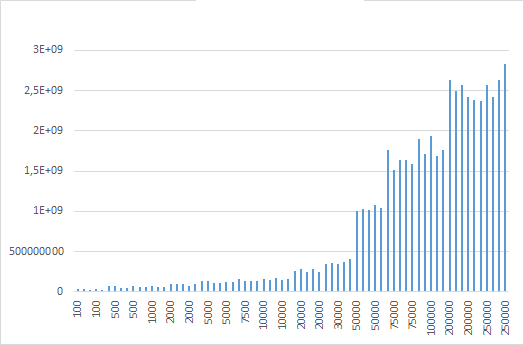
\includegraphics[width=150mm, frame]{images/LIKEE-1-CREATE-ALL.png}
\caption{LIKEE-1-CREATE-ALL - 5x měřená hodnota pro každou velikost tabulky - Vertikální osa čas $10^{-9}$ sekund a horozontální značí velikosti tabulek.}
\label{sec:obr1}
\end{figure}

\paragraph{Normální rozložení} Potřebovali jsme na základě těchto hodnot vytvořit funkce podle kterých, by jsme mohli určit přibližnou hodnotu různě velkých tabulek, pro které nemáme hodnoty naměřené. Na základě měření jsme rozhodli, že veškeré měřené hodnoty mají normálního rozložení (například tabulka o velikosti 100, nad kterou byl volán Select všech rádků (viz. obrázek \textbf{číslo \ref{sec:obr3}}).
U každého jednotlivého grafu znázorňující naměřené hodnoty (viz. obrázek\ref{sec:obr1}) bylo zapotřebí zvážit zda není vhodné ho rozdělit na více intervalů, kde by  vytvořená funkce počítala přesněji. Z hodnot ze zvoleného intervalu jsme přes online nástroj pro vytváření polynomu viz. \cite{polregres} vždy získali dány polynom většinou čtvrtého řádu, do kterého jsme potom dosadili původní velikosti tabulek. Původní graf hodnot a hodnoty z nových funkcí jsme si dali dohromady do grafu na porovnání. Na obrázku \textbf{číslo \ref{sec:obr2}} můžeme vidět jak žlutá barva znázorňuje body spočítané z nově vytvořených funkcí. 

\begin{figure}[H]
\centering
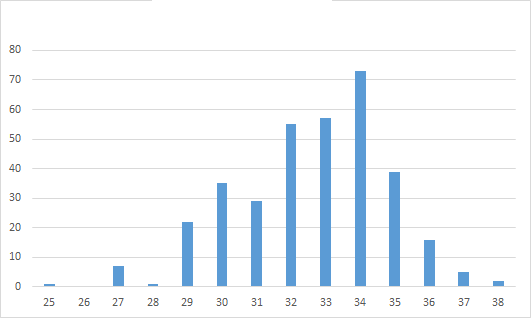
\includegraphics[width=150mm, frame]{images/100-TABLE-SELECT-ALL-342.png}
\caption{100-TABLE-SELECT-ALL - rozložení při 342 měřeních - vertikální osa značí počet výskytů a horozontální značí $10^{-2}$ sekund zaokrouhleno na celá čísla}
\label{sec:obr3}
\end{figure}

\begin{figure}[H]
\centering
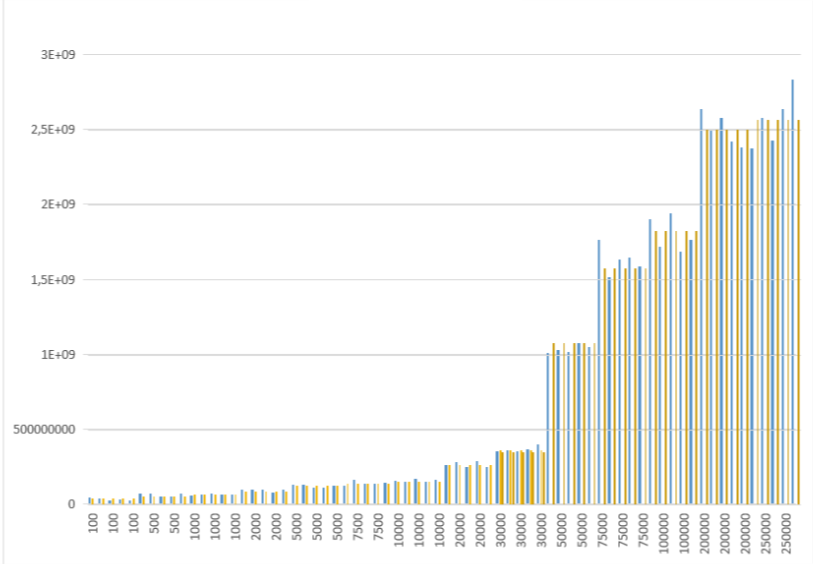
\includegraphics[width=150mm, frame]{images/LIKEE-1-CREATE-ALL-FUNCTIONS.png}
\caption{LIKEE-1-CREATE-ALL-FUNCTIONS - 5x měřená hodnota pro každou velikost tabulky - Vertikální osa čas $10^{-3}$ sekund a horozontální značí velikosti tabulek.}
\label{sec:obr2}
\end{figure}

\paragraph{DX - odchylka} Pro jednotlivé intervaly jsme si u každého bodu co jsme měli naměřenou hodnotu spočítali hodnotu funkce, porovnali s naměřenou hodnotou, a tím zjistili chybu v jednotlivých bodech. Tyto chyby stačilo zprůměrovat a získali jsme hodnotu odchylky. 

\paragraph{EX - Střední hodnota} Střední hodnotu jsme zjistili z funkcí  aproximovaných z naměřených hodnot (obrázek \textbf{číslo \ref{sec:obr9}}). Tato funkce nám potom vypočítávala pro danou velikost tabulky její střední hodnotu.

\begin{figure}[H]
\centering
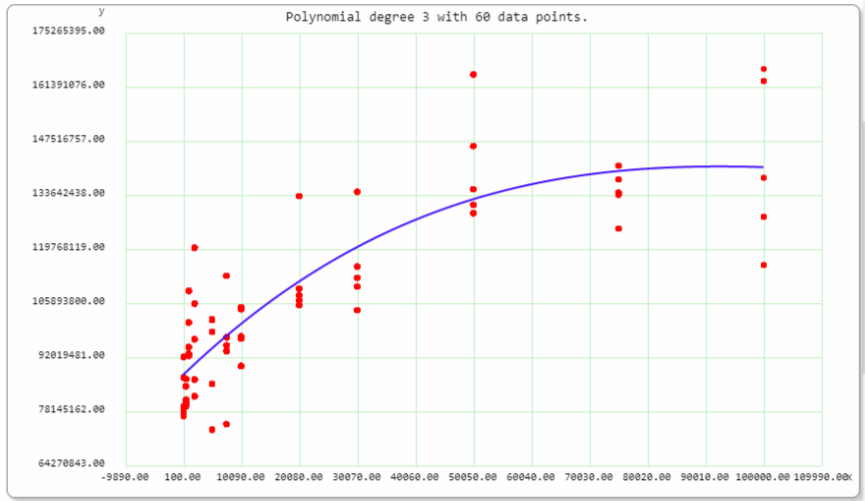
\includegraphics[width=150mm, frame]{images/VYPOCET-KRIVEK.png}
\caption{Příklad proložení naměřených hodnot krivkou zapoužítí online nástroje \textit{arachnoid} \cite{polysolv} při vytváření polynomů}
\label{sec:obr9}
\end{figure}

\section{Koncepce modelu}


\subsection{Komunikace JAVA a databáze}
Na obrázcích \textbf{č. \ref{sec:obr8}} a \textbf{č. \ref{sec:obr10}} je znázorněna komunikace mezi JAVou a databází za pomoci JDBC - API pro programovací jazyk Java, který definuje jednotné rozhraní pro přístup k relačním databázím \cite{connectivity}. Pro přístup ke konkrétnímu databázovému serveru je potřeba JDBC driver (ovladač), který poskytuje tvůrce databázového serveru. Pro náši PostgreSQL databázi dostupný na oficiálních stránkách \cite{jdbc}.

\begin{figure}[H]
\centering
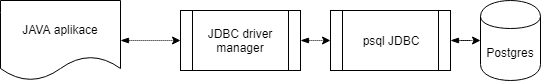
\includegraphics[width=150mm]{images/JAVA-DB-komunikace.png}
\caption{Komunikace JAVA-DB}
\label{sec:obr8}
\end{figure}

\begin{figure}[H]
\centering
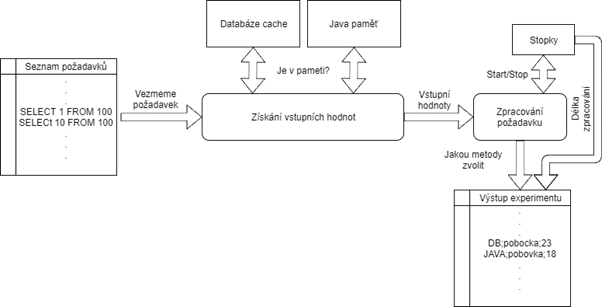
\includegraphics[width=150mm]{images/JAVA-DB-schema.png}
\caption{Schéma JAVA-DB}
\label{sec:obr10}
\end{figure}

\subsection{Simulace experimentu} 
	%Simulace experimentu je popsána na obrázku (<<obrázek experimentu>>).
	 Jednotlvé experimenty (viz. kapitola \textbf{Experimenty \ref{sec:experimenty}}) nám představují seznam požadavků (viz. kapitola \textbf{Experimenty vysvětlení požadavků \ref{sec:experimenty}}). 
	Bereme postupně požadavky a získáváme informace o velikosti tabulky a přesnosti filtrování viz. \textbf{LIKEE \ref{sec:likee}}. Na základě těchto informací se zeptáme jestli je tato tabulka v cache databáze a jestli je v paměti JAVY. Tyto čtyři hodnoty pak pošleme do procesu na zpracování jednoho požadavku. Stopujeme si čas jak dlouho trvá pro JAVU a Databázi zpracování požadavku. Jednotlivé doby trvání zpracování požadavku dáváme do výstupního souboru pro daný experimentu. % U některých experimentů jsou i na konci sumy (<<definice sumy>>) pro jednotlivé metody k porovnání.


\subsection{Architektůra sim modelu}
Simulační model byl napsán v jazyce C++\cite{c++} za pomocí simulační knihovny Simlib\cite{simlib_web, simlib_zdroj}. Dále popsáno v kapitole \textbf{Simlib \ref{sec:simlib}}.

\subsection{Konceptuálního modelu na simulační}
Simulační model je vytvořen na základě modelu přistupování do databázového serveru běžně používaném v reálném světě. V našem projektu jsme pracovali pouze s daty z virtuální verze, ve které jsme se snažili co nejpřesněji reálný systém imitovat.

\subsubsection{Mapování konceptuálního modelu na simulační}
\begin{center}
\begin{tabular}{ |l|l| }
  \hline
  \textbf{Konceptuální model} &  \textbf{Procedůra} \\ \hline      \textbf{Databáze} &  \textbf{DB\_* procedůry (...)} \\ \hline 
  Vytváření objektů & Proces\_create\_objects \\ \hline
  Select radku z DB First & Proces\_select\_for\_first\_time \\ \hline
  Select radku z DB N & Proces\_select\_N \\ \hline
  FIltrace v Javě & Proces\_filter\_objects\\ \hline
\end{tabular}
\end{center}

\subsection{Zpracování požadavku}
	Zpracování jednoho požadavku máme znázorněné na Petriho síťi (viz.
	IMS - Modelovani a simulace - strana 123. \cite{ims-prednasky}) (\textbf{Petriho sítě Obr. č. \ref{sec:obr7}}). Toto zpracování nám pouze určuje jakou metodu filtrace dat(výběr mezi JAVA a Databází), bychom měli zvolit pro vstupní hodnoty. 
\\
Význam vstupních hodnot:

\begin{itemize}
\item Přesnost filtrace: jaký LIKEE je daný požadavek
\item Velikost tabulky: počet řádků vstupní tabulky
\item Tabulka je v ram. JAVA: říká nám jestli je tabulka nacacheovaná v paměti JAVy
\item Tabulka je v ram. Databáze: určuje jestli je tabulka nacacheovaná v paměti databáze

\end{itemize}

\subsection{Petriho sít} \label{petrinetwork}
Naše petriho sít (Obr . č. \ref{sec:obr7}) je pouhým zjednodušeným modelem simulace. Při tvorbě skutečné simulace jsme sice vycházeli z toho to návrhu, ale trošku se nám liší (viz. kapitola \textbf{Simlib \ref{sec:simlib}}). 

V obrázku Petriho sítě(Obr . č. \ref{sec:obr7}) máme zakresleno, že nám vstupní hodnoty Přesnost filtrace a Velikost tabulky vstupují do přechodu s názvem Výběr z DB / Vytváření objektů / Filtrace v JAVě. Znamená to, že tyto vstupní hodnoty použijeme při zjišťování doby konání těchto přechodů.

Pokud máme hodnoty Tabulka je v pam. JAVě a Tabulka je v pam. databáze zadané, tak se nám vygenerují dva procesy.

Procesy Start/Stop stopky pro Javu a Databáni nám určují místo kdy se začne měřit čas potřebný pro zpracování požadavku, pro danou metodu.

Na začátku petriho sítě (Obr. \textbf{č. \ref{sec:obr7}}) nám vznikne jeden proces v \textbf{Požadavek}. Ten se rozdělí na dva procesy, jeden bude představovat zpracování Javou a druhý zpracování databází.
Na základě vstupních požadavků jsou vykonány pro JAVU a databázi rozdílné přechody. Na příklad pokud máme na vstupu dáno, že je tabulka v paměti databáze, tak se vykoná proces SELECT (N). Jakmile se proces pro JAVU a databázi dokončí, zastaví stopky a pokud skončil jako první, tak přejde do stavu Zvolit. Stavy Zvolit máme dva, jeden pro každou metodu.  Jde zvolit vždy jen jeden z těchto dvou stavů. Dozvíme se tak, kterou z těchto dvou metod máme zvolit.
Jednotlivé přechody a jejich významy jsou vysvětleny v kapitole \textbf{Simlib \ref{sec:simlib}}.

\paragraph{Filtrování} Filtrování \textbf{JAVA} se skládá ze tří částí:

\begin{itemize}
\item SELECT (first) - případ, kdy databáze ještě nemá tabulku v paměti cache (nevyužívá přesnosti)
\item SELECT (N) - databáze již má tabulku v paměti (nevyužívá přesnoti)
\item SELECT (N) - databáze již má tabulku v paměti (využívá přesnoti)
\end{itemize}


Filtrování \textbf{Databáze} (SQL dotazy) je složena ze dvou částí:

\begin{itemize}
\item SELECT (first) (přesnost) - je stajná jako u filtrace v Javě, je s rozdílem, že využívá přesnosti
\item SELECT (N) (přesnost) - také ještě navíc využívá přesnosti
\end{itemize}


\newpage
\begin{figure}[H]
\centering
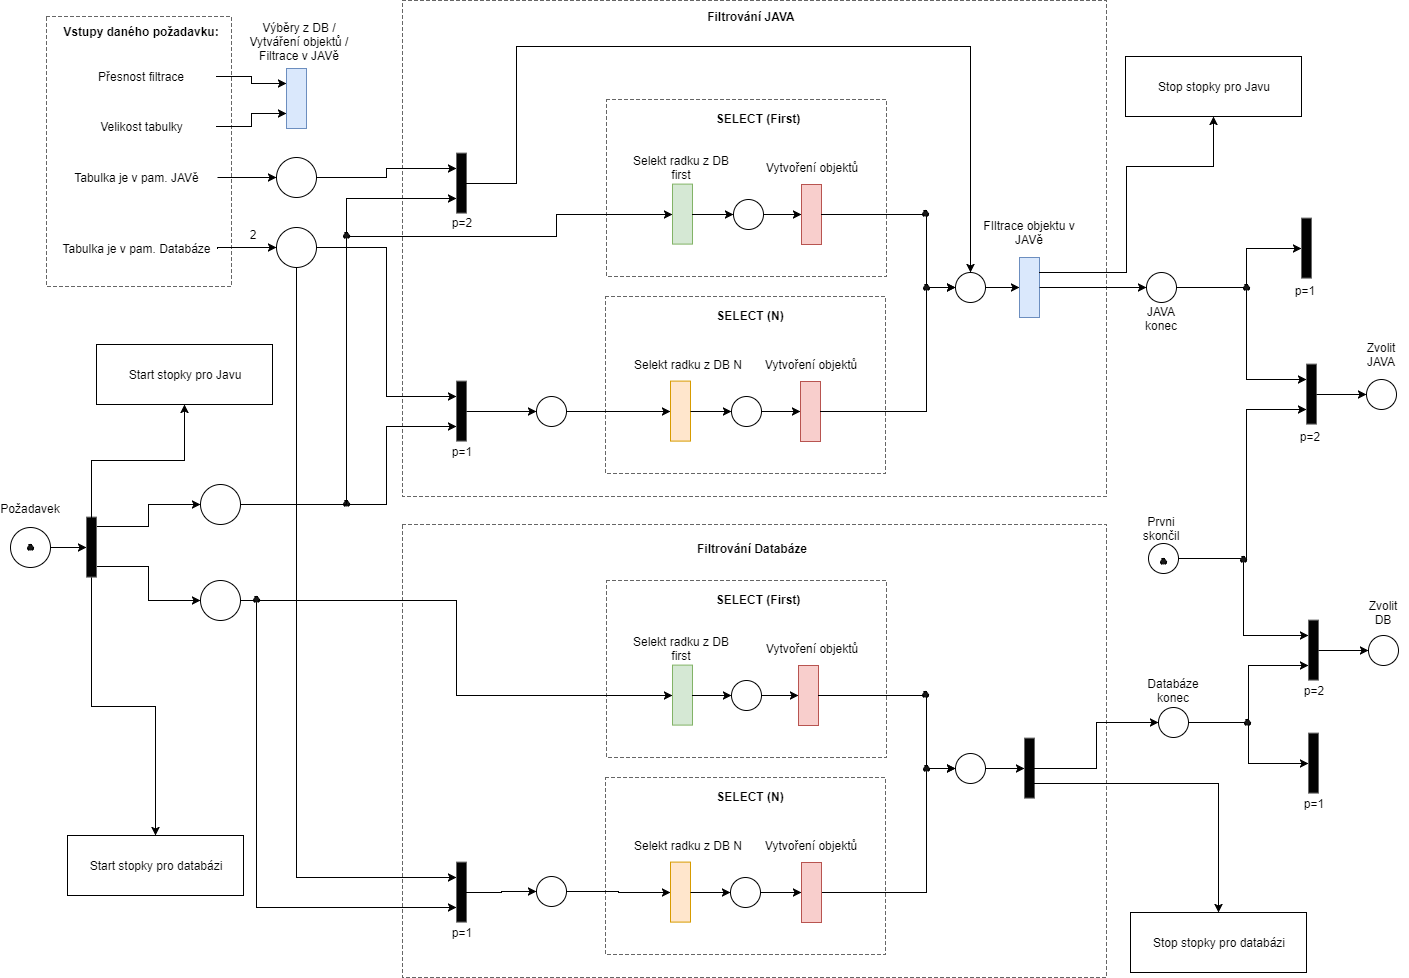
\includegraphics[width=220mm,  angle =90]{images/IMS-projekt.png}
\caption{Petriho sít}
\label{sec:obr7}
\end{figure}
\newpage

\section{Simlib} \label{sec:simlib}
Program v simlibu\cite{simlib_web, simlib_zdroj} je rozdělen na dvě hlavní větve znázorňující model pro filtraci dat přes JAVu a přes Databázový server. Jednotlivé doby vyhledání jsou zakresleny a jejich průběhy popsány v kapitole \textbf{Petriho síte \ref{petrinetwork}}. Na začátku programu se na základě předem určených dat, nad kterými se budou provádět simulace (zvolených experimentů) vytvoří fronty pro větve Javy a databáze. Na základě hodnot spočítaných z funkcí, které jsme získali při analýze vstupních dat (viz. kapitola \textbf{Zpracování naměřených hodnot \ref{zprachodnot}}) propočítáváme doby trvání.

\section{Experimenty} \label{sec:experimenty}
\subsection{Podstata simulačních experimentů a jejich průběh}
Vytvořili jsme několik experimentů. Chceme na nich ukázat, při jakých parametrech se vyplatí filtrovat data v databázi a kdy se nám vyplatí si načíst celou tabulku a data si pak filtrovat v javě.

\subsection{Příklady}

\subsubsection{SELECT FIRST MEMORY}
Na obrázcích \ref{sec:obr5}, \ref{sec:obr6}, \ref{sec:obr4} jsou znázorněny průběhy dob vyhledávání v JAVA oproti Databázi. Jedná se o experiment s nenacachovanými hodnotami (FIRST). Na obrázcích můžeme videt jak se jednotlivé selecty chovají. JAVA jelikož není nacachovaná bude pro filtraci  s jakoukoliv přesností mít velice podobný průběh. Databáze ovšem jasně znázorňuje, že čas za který, při přesnějším vyhledávání, proběhne je mnohem menší.

\begin{figure}[H]
\centering
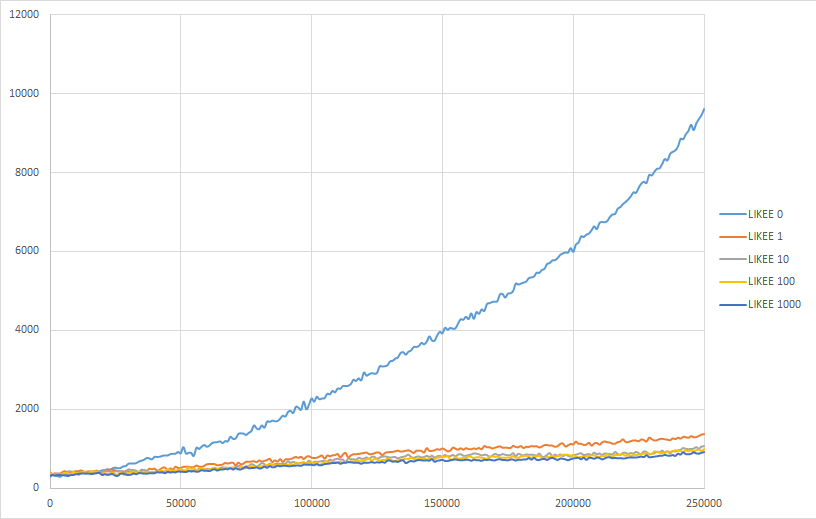
\includegraphics[width=150mm, frame]{images/FIRST-DB.png}
\caption{FIRST - DB - LIKEE 0-1-10-100-1000 - Vertikální osa čas $10^{-3}$ sekund a horozontální značí velikosti tabulek.}
\label{sec:obr5}
\end{figure}

\begin{figure}[H]
\centering
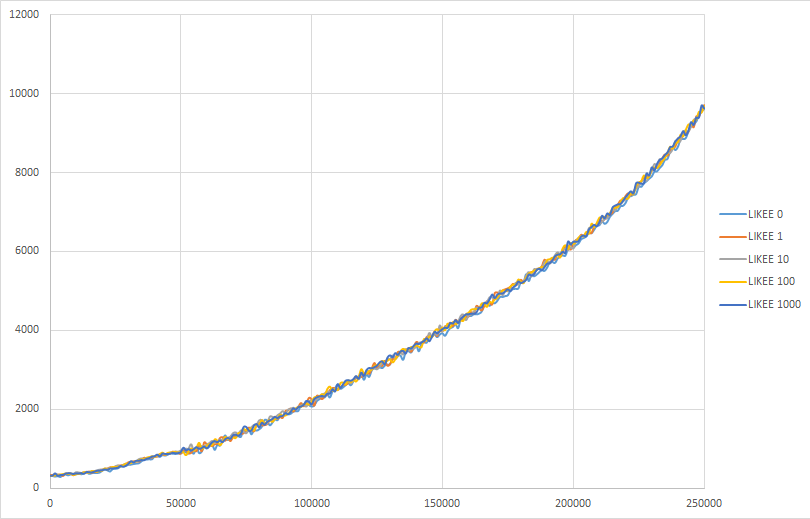
\includegraphics[width=150mm, frame]{images/FIRST-JAVA.png}
\caption{FIRST - JAVA - LIKEE 0-1-10-100-1000 - Vertikální osa čas $10^{-3}$ sekund a horozontální značí velikosti tabulek.}
\label{sec:obr6}
\end{figure}

\begin{figure}[H]
\centering
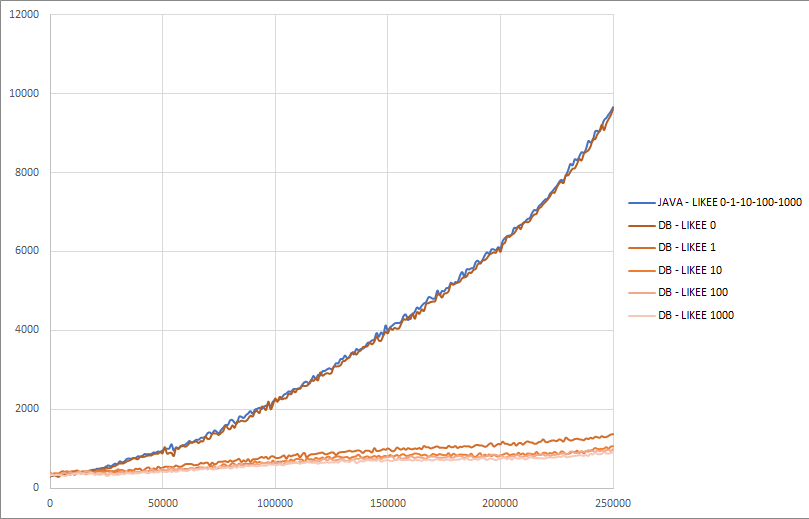
\includegraphics[width=150mm, frame]{images/FIRST-DB-JAVA-INTERSECTION.png}
\caption{FIRST - DB AND JAVA - LIKEE 0-1-10-100-1000 TABLE 0-40000 - Vertikální osa čas $10^{-3}$ sekund a horozontální značí velikosti tabulek.}
\label{sec:obr4}
\end{figure}


	
\subsubsection{Příklad ze života}
Tento experiment jsme vytvářeli jako příklad z nějakého většího systému. Předpokládáme, že máme nějakou firmu, která má spousty zaměstnanců a my potřebujeme vyhledat informace o jednom zaměstnanci. Víme, kde pracuje a jakou má pozici.
 
Na začátku si zobrazíme všechny pobočky. %V našem případě tabulka s <<množina řádků>>. 
Potom si pomoci filtrace najdeme určitou pobočku, zobrazíme si informace o pobočce. Vybereme si jednoho zaměstnance. Zobrazíme si opět všechny pobočky.
V kódu experimentu to pak bude vypadat následovně:
  

Vypsani všech poboček:
\begin{itemize}
\item     {39000, 0},  //LIKEE(0) = SELECT vsech řádků tabulky
\end{itemize}

Vybrani jedne pobočky:
\begin{itemize}
\item {39000, 1000}, 
\end{itemize}

Zobrazení informací o pobočce
\begin{itemize}
\item     {100, 100},             // dohledani nazvu prodejny
\item     {500, 10},              // dohledani zamestnancu na prodejne
\item     {451, 10},              // dohledani dalsich informaci
\item     {452, 10},              // dohledani dalsich informaci
\item     {453, 10},              // dohledani dalsich informaci
\end{itemize}

Vypsání opět všech poboček:
\begin{itemize}
\item     {39000, 0}, //LIKEE(0) = SELECT vsech řádků tabulky
\end{itemize}

\subsubsection{Další:}
\begin{itemize}
\item Obecný - Máme velkou tabulku a z ní si pak filtrujeme
\item Pouze jedna opravdu velkou
\item filtrace velké tabulky - ale z nich jen malá data
\item Smíšený
\item Zátěžový - spoustu velký tabulek
\item Spoustu nejpřesnějších informací
\end{itemize}

%vytvořili jsme si jednotlivé testovací příkjhasdfjkdfjk
%5.2 - dokumentace jednotlivých experimentů
%	Experiment 1-N
%	Obecná simulace
%	Přesná simulace
%	¨Náhodná simulace¨
%	Experimentu na jedné tabulce
%	Závěry z těchto experimentů

\subsection{Výsledky/Grafy}
Vzhledem k tomu, že jsme zjistili chybu ve sběru dat, musíme s lítostí přeskočit prezentaci výsledků a grafů, jelikož by vyvozovali závěry neodpovídající reálnému systému.

\section{Závěr}
Na základě výsledků z předběžných měřeních jsme očekávali, že filtrování pomocí databáze se má vyplatit u tabulek větších než 70 000 řádků. Tuto hodnotu jsme odhadovali na základě \textbf{Obr. č. \ref{sec:obr11}}, kterou jsme naměřili při prvotním měření dat v systému s jinými parametry. Považujeme ji za správnou, jelikož logicky Databázové SQL SELECTY musí filtrovat být při větším počtu řádků v tabulce mnohem efektivněji, protože nemusí se přenášet veškerá data jako JAVA.

\begin{figure}[H]
\centering
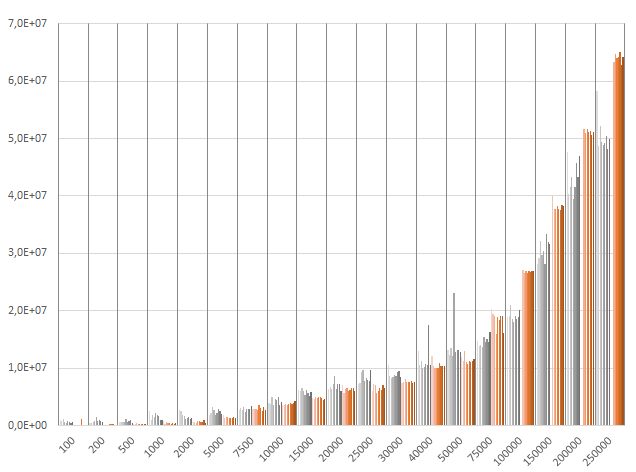
\includegraphics[width=150mm, frame]{images/JAVA-DB-prolnuti.png}
\caption{JAVA - oranžová, DB - šedá | Vertikální osa čas $10^{-6}$ sekund a horozontální značí velikosti tabulek.}
\label{sec:obr11}
\end{figure}

Po provedení našich simulací, se nám toto tvrzení nepodařilo prokázat. Následně jsme zjistili, že je to zapříčiněno chybou v měření. Chybu jsme zpětně nalezli ve špatném postupu měření dob. Chyba byla způsobena rychlostí disku. Virtuální počítače, na kterých probíhal sběr dat, se navzájem přetahovali o přístup do disku.

%Na závěr bychom chtěli doplnit, že námi napsaný program, napsaný v jazyce C++ s připojenou knihovnou Sim 

Předpokládáme, to že kdybychom našemu simulačnímu programu dali přesnější vstupní data, tak by jsme dosáhli výsledků odpovídajícím hodnotám reálného systému.


\pagebreak
\newpage
\bibliographystyle{czechiso}
\def\refname{Literatura}
\bibliography{proj4}

\end{document}